\section{Аналитический раздел}
\subsection{Задача оценки безопасности водителя}
Оценка безопасности водителя -- это комплексная задача, нацеленная на анализ действий водителя. В последнее время большое внимание уделяется разработке интеллектуальных систем, способных автоматически оценивать уровень внимания водителя. Основным источником данных для таких систем часто выступают фото или видео, получаемые с камер из салона автомобиля направленных на водителя. Таким образом, основной частью задачи оценки безопасности водителя является задача классификации изображений, где основные классы -- это различные состояния водителя, например, <<смотрит на дорогу>>, <<пьет воду>>, <<смотрит в телефон>> и так далее. После шага классификации всех изображений, можно вычислить оценку безопасности водителя проанализировав количество тех или иных классов.

\subsection{Задача классификации изображений}
Задачи классификации -- это задачи, в которых объект должен быть отнесен к одному из $n$ классов на основе индекса сходства его характеристик с каждым классом. Под классами понимается набор подобных объектов. Объекты
считаются похожими на основе совпадающих характеристик, таких как цвет, форма, размер и т.д. Классы определяются на основе их уникальных меток. В частности, задача «распознавания действий человека за рулем автомобиля по фото» является задачей классификации изображений.

Основным алгоритмом для решения задачи классификации изображения являются глубокие нейронные сети, а именно сверточные нейронные сети (CNN).

\subsection{Введение в сверточные нейронные сети}
\subsubsection{Нейрон}

Биологическая нервная система представляет собой сеть, состоящую из множества нейронов. Аналогичным образом, нейроны также являются основным процессорным блоком искусственных нейронных сетей. Принцип работы заключается в том, что множество входных значений подвергаются математическому преобразованию для получения выходного значения (рисунок \ref{fig:neuron}). Соотношение математического преобразования между входным сигналом и выходным значением представлено формулой:

\begin{equation}
f(b + \sum_{i=1}^{n}(x_i \times w_i),
\end{equation}

где $f$ -- функция активации, например ReLU, Sigmoid, Tanh и другие.

\begin{figure}[hbtp]
	\centering
	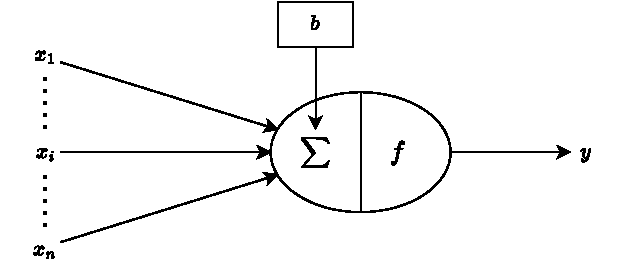
\includegraphics[width=\textwidth]{img/neuron.pdf}
	\caption{Модель нейрона.}
	\label{fig:neuron}
\end{figure}




\subsubsection{Многослойный персептрон}

Многослойный персептрон состоит из входного слоя, скрытого слоя (одного или нескольких) и выходного слоя. Он содержит несколько базовых модульных нейронов, которые осуществляют передачу сигнала посредством послойной проводимости между нейронами. На рисунке \ref{fig:mlp} приведен пример структуры MLP. $H$ -- вектор выходного значения скрытого модуля $H=F(W_{h}X+B_h)$, $Y$ -- вектор выходного значения выходного модуля $Y=F(W_{y}H+B_y)$, где $X$ -- матрица входных значений, $W_h$ и $W_y$ матрица весов между слоями, $B_h$ $B_y$ -- матрицы смещения.

\begin{figure}[hbtp]
	\centering
	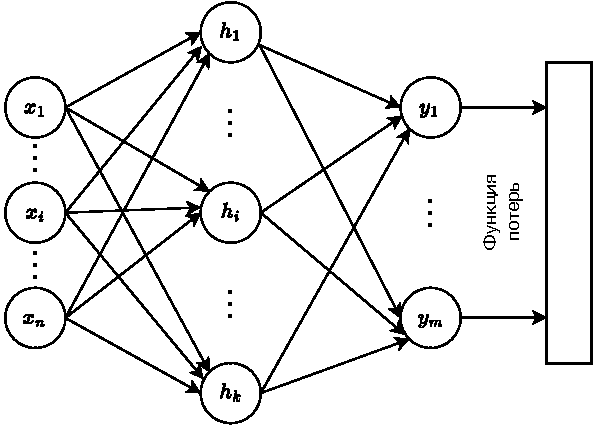
\includegraphics[width=\textwidth]{img/mlp.pdf}
	\caption{Структура многослойного персептрона.}
	\label{fig:mlp}
\end{figure}


\subsection{Архитектура сверточных нейронных сетей}

Основная структура CNN включает сверточный слой, слой пулинга, слой нелинейной активации и полносвязный слой. Изображение сначала предварительно обрабатывается и подается на вход сети, где проходит через чередующиеся слои свертки и пулинга, после чего классифицируется полносвязным слоем. 

CNN дополняют структуру MLP за счет введения сверточных и слоев пулинга, что дает преимущества в обработке изображений с большим количеством пикселей и в больших наборах данных, обеспечивая лучший размер модели и производительность \cite{cnn-mlp}. Сверточный слой обладает свойствами локального рецептивного поля, сохраняя форму входного изображения и эффективно распознавая взаимосвязь между пикселями по длине и ширине за счет использования параметрического разделения и разреженной связи. Слой пулинга уменьшает вычислительную нагрузку и чувствительность к положению, способствуя инвариантности к перемещению, масштабированию и искажениям входных изображений.

\subsubsection{Сверточный слой}

Для сверточных нейронных сетей определенной глубины операция свертки нескольких сверточных слоев может извлекать различные характеристики входного сигнала. Нижний слой свертки обычно извлекает общие характеристики, такие как текстуры, линии и грани, в то время как более высокие слои извлекают более абстрактные признаки.

Сверточный слой имеет несколько сверточных ядер с обучаемыми параметрами. Это матрица, составленная из обучаемых весов, которые обычно имеют размеры $3 \times 3$, $5 \times 5$ и $7 \times 7$ с равной длиной, шириной и нечетным числом. Обычно сверточный слой  принимает карты признаков (feature maps). Матрица весов ядра свертки соответствует локальной области карты объектов-соединений, и ядро свертки последовательно выполняет операции свертки над областью на карте \cite{conv-layer}.

Как правило, размеры входных карт $H \times W \times C$
(высотой $H$, шириной $W$ и каналы $C$), каждое ядро свертки $K \times K \times C$
это число ядра свертки должна быть такой же, как число входных каналов. На рисунке \ref{fig:conv_layer} представлена  схема процесса свертки входных карт объектов ($5 \times 5 \times 3$) и ядра свертки ($3 \times 3 \times 3$). Поток данных в сверточном слое можно приблизительно выразить как:

\begin{equation}
feature\_surface_{out} = f\left(\sum_{i = 3}^3M_i \ast W_i + B\right),
\end{equation}

где $M_i$ представляет собой поверхность объекта входных карт объектов,  $W_i$ -- матрица весов ядра свертки, $M$ - матрица смещения, $f(\cdot)$ -- нелинейная функция активации, а $feature\_surface_{out}$ выходная карта признаков.

\begin{figure}[hbtp]
	\centering
	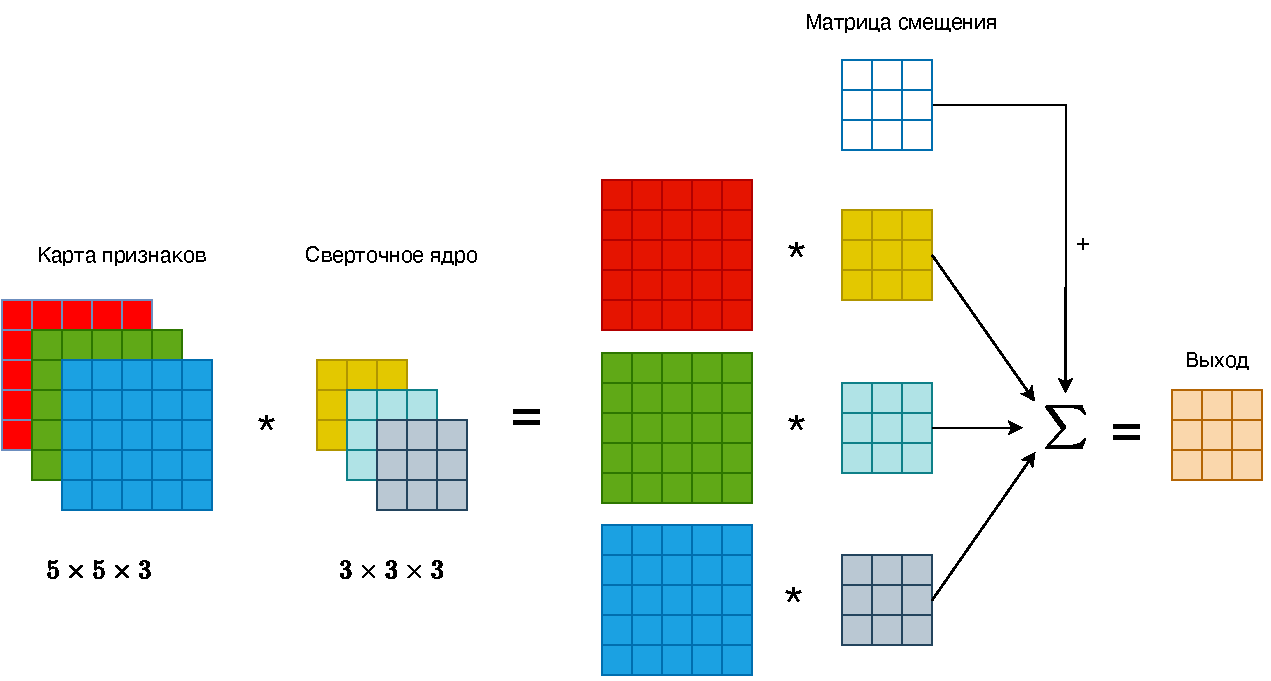
\includegraphics[width=\textwidth]{img/conv_layer.pdf}
	\caption{Схематичная диаграмма процесса свертки.}
	\label{fig:conv_layer}
\end{figure}

\textbf{Слой активации}
Скалярный результат каждой свёртки попадает на функцию активации, которая представляет собой некую нелинейную функцию. Слой активации обычно логически объединяют со слоем свёртки (считают, что функция активации встроена в слой свёртки). 

Функция активации решает, следует активировать нейрон или нет. Это означает, что она будет решать, важен или нет вход нейрона в сеть в процессе прогнозирования. На данный момент в качестве функции активации используются ReLU (сокращение от англ. rectified linear unit) функции, такие как ReLU, Leaky ReLU, PReLU, RReLU и ELU \cite{relu}.


\subsubsection{Слой пулинга}

Пулинг-слои обычно следуют за сверточными слоями. Основные причины использования пулинг-слоя:
\begin{itemize}[leftmargin=1.6\parindent]
	\item[--] выполнение процесса субдискретизации и уменьшения размерности входного изображения для уменьшения количества соединений сверточного слоя, что в свою очередь снижает вычислительную нагрузку сети \cite{pooling-layer-1};
	\item[--] обеспечение инвариантности к масштабированию, сдвигу и повороту входного изображения\cite{pooling-layer-2};
	\item[--] обеспечение более устойчивой работы выходной карты признаков к искажениям и ошибкам отдельного нейрона \cite{pooling-layer-3}.
\end{itemize}

Наиболее широко используемыми методами пулинга являются средний и максимальный пулинг \cite{pooling-layer-4}.
На рисунке \ref{fig:pooling-layer} показан процесс субдискретизации максимального и среднего пулинга.

\begin{figure}[hbtp]
	\centering
	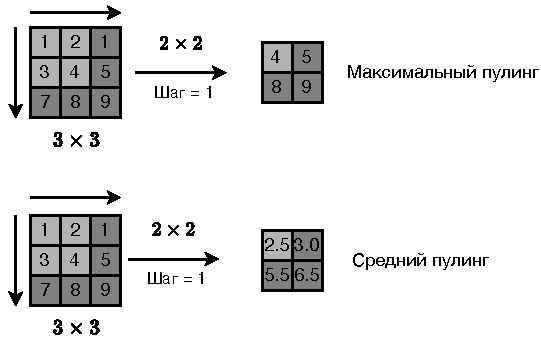
\includegraphics[width=\textwidth]{img/pooling.pdf}
	\caption{Максимальный и средний пулинг.}
	\label{fig:pooling-layer}
\end{figure}

\clearpage


\subsubsection{Полносвязный слой}
Полносвязный  слой обычно находится после непрерывного сверточного слоя и слоя пулинга. Он интегрирует и классифицирует локальную информацию, извлеченную после свертки и пулинга и в конечном итоге выводит информацию о категории изображения. 

Он содержит несколько скрытых слоев, которые извлекают высокоуровневые признаки из предыдущей сети в более сложной форме. Количество нейронов на выходном конце равно количеству категорий. Затем выходной вектор используется для определения принадлежности изображения к категории. Проще говоря, полносвязный слой действует как классификатор в сверточной нейронной сети.

Во время обучения  выход сети обычно подвергается softmax регрессии\cite{pooling-layer-1} для нормализации вероятности перед функцией потерь полносвязного слоя. Параметры слоя обновляются с использованием обратного распространения градиента.

\subsubsection{Функция потерь}
В дополнение к различным типам слоёв архитектуры сверточных нейронных сетей, которые были представлены в выше, окончательная классификация достигается с помощью выходного слоя, который обычно является последним слоем полносвязного слоя. Разные функции потерь оказывают влияние на производительность архитектуры CNN и применяются для различных задач, таких как классификация изображений, распознавание лиц и объектов.

\newpage
\subsection{Технологии классификации изображений}
Для решения задачи классификации изображений используются такие модели сверточных сетей, как\cite{models-comprasion}: 
\begin{itemize}[leftmargin=1.6\parindent]
	\item[--] AlexNet;
	\item[--] VGGNet;
	\item[--] GoogleNet;
	\item[--] ResNet.
\end{itemize}

\subsubsection{AlexNet}
 AlexNet имеет восьмислойную структуру: первые пять слоев являются сверточными, а последние три полносвязными. Для выполнения обучения сети требуется изображение с разрешением $227 \times 227$ в качестве входных данных и информация о классификации, встроенная в изображение в качестве выходных данных.
 
Принцип работы AlexNet представлен на рисунке \ref{fig:alexnet}.

\begin{figure}[hbtp]
	\centering
	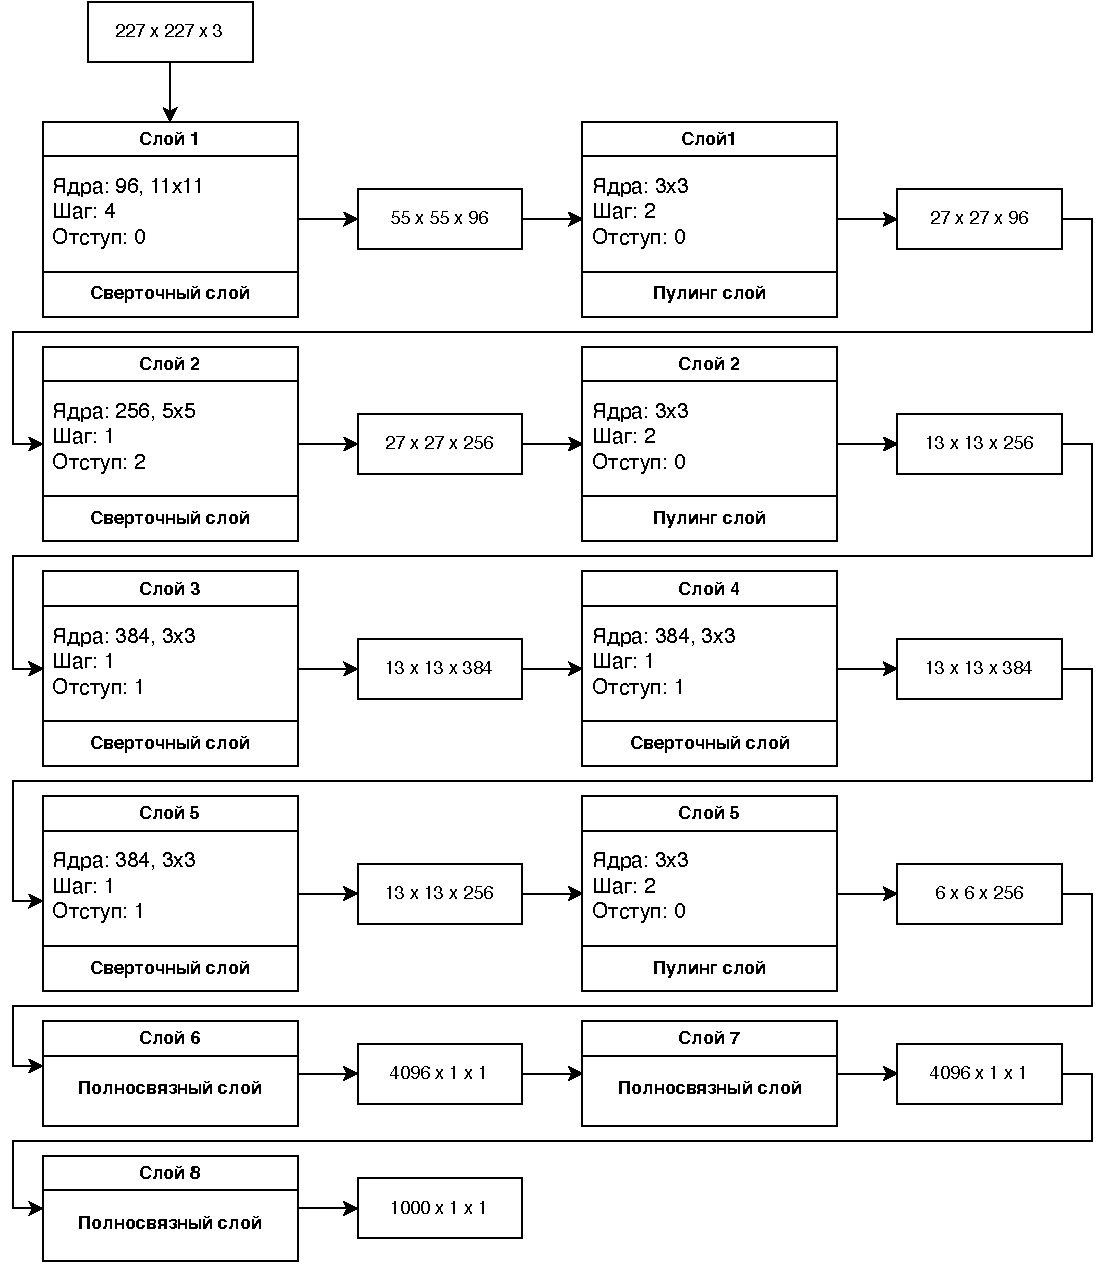
\includegraphics[width=\textwidth]{img/alexnet.pdf}
	\caption{Принцип работы AlexNet}
	\label{fig:alexnet}
\end{figure}
\clearpage

\subsubsection{VGGNet}
Эта модель аналогична модели AlexNet и также использует структуру области сверточных слоев, за которой следует область полносвязных слоев. Правило компоновки модуля VGG заключается в последовательном использовании нескольких идентичных сверточных слоев, за которыми следует слой максимального пулинга, при этом сверточный слой сохраняет высоту и ширину входных данных неизменными, в то время как пулинг слой уменьшает их вдвое. 

Сеть VGG имеет множество различных моделей, одной из которых является VGG-16, принцип работы которой изображен на рисунке \ref{fig:vggnet}. Она содержит 16 уровней весов, сеть последовательно соединяет пять блоков, и в конце подключаются два полносвязных слоя с 4096 и выходной слой с 1000 классами.

\begin{figure}[hbtp]
	\centering
	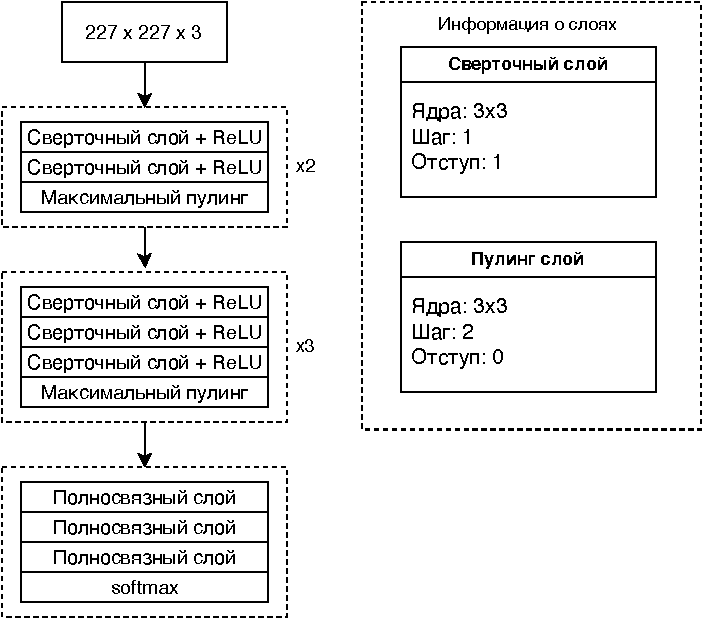
\includegraphics[width=\textwidth]{img/VGGNet.pdf}
	\caption{Принцип работы VGG-16}
	\label{fig:vggnet}
\end{figure}
\clearpage


\subsubsection{GoogleNet}
GoogleNet изменила структуру CNN, введя параллельное внутреннее соединение с помощью структуры $Inception$. Как показано на рисунке \ref{fig:inception}, когда данные обрабатываются с использованием $inception$, они должны одновременно проходить через четыре пути с различными сверточными ядрами; в итоге данные объединяются в новый слой сети. Структура $inception$ является самым значительным отличием GoogleNet от традиционных сетей CNN. Существует 4 разновидности структуры: $inceptionV1$, $inceptionV2$, $inceptionV4$, $inceptionV4$ \cite{googlenet}, в данной работе рассматривается первая вариация.

Использование структуры $inception$ имеет два основных преимущества: во-первых, одновременное свертывание на нескольких масштабах позволяет извлекать характеристики на разных масштабах, что также приводит к большей точности в окончательном классификационном суждении; второе – использование свертки 1×1 для сокращения размерности позволяет уменьшить вычислительную сложность, и объем вычислений значительно сокращается, когда уменьшается количество признаков, после чего выполняется свертывание. Благодаря преимуществам $inception$, хотя у GoogleNet 22 слоя сети, что глубже, чем 8 слоев у AlexNet или 19 слоев у VGGNet, она может достичь гораздо большей точности, чем AlexNet, имея только 5 миллионов параметров (1/12 от параметров AlexNet и 1/25 от параметров VGG-16) \cite{googlenet}.

На рисунке \ref{fig:googlenet} представлен принцип работы GoogleNet, на рисунке присутствуют $Stem$ блок и блок вспомогательного классификатора.

$Stem$ блок является фундаментов модели, он основан на идее, что перед тем как данные будут переданы через серию  $Inception$-блоков, первоначальное представление входных данных должно быть наиболее эффективно обработано для дальнейшего извлечения признаков. 

Блок вспомогательного классификатора вводится в качестве дополнительного средства для улучшения обучающих характеристик глубоких нейронных сетей.

Структуры $Stem$ блока и вспомогательного классификатора представлена на рисунке \ref{fig:stem_aux}.

\begin{figure}[hbtp]
	\centering
	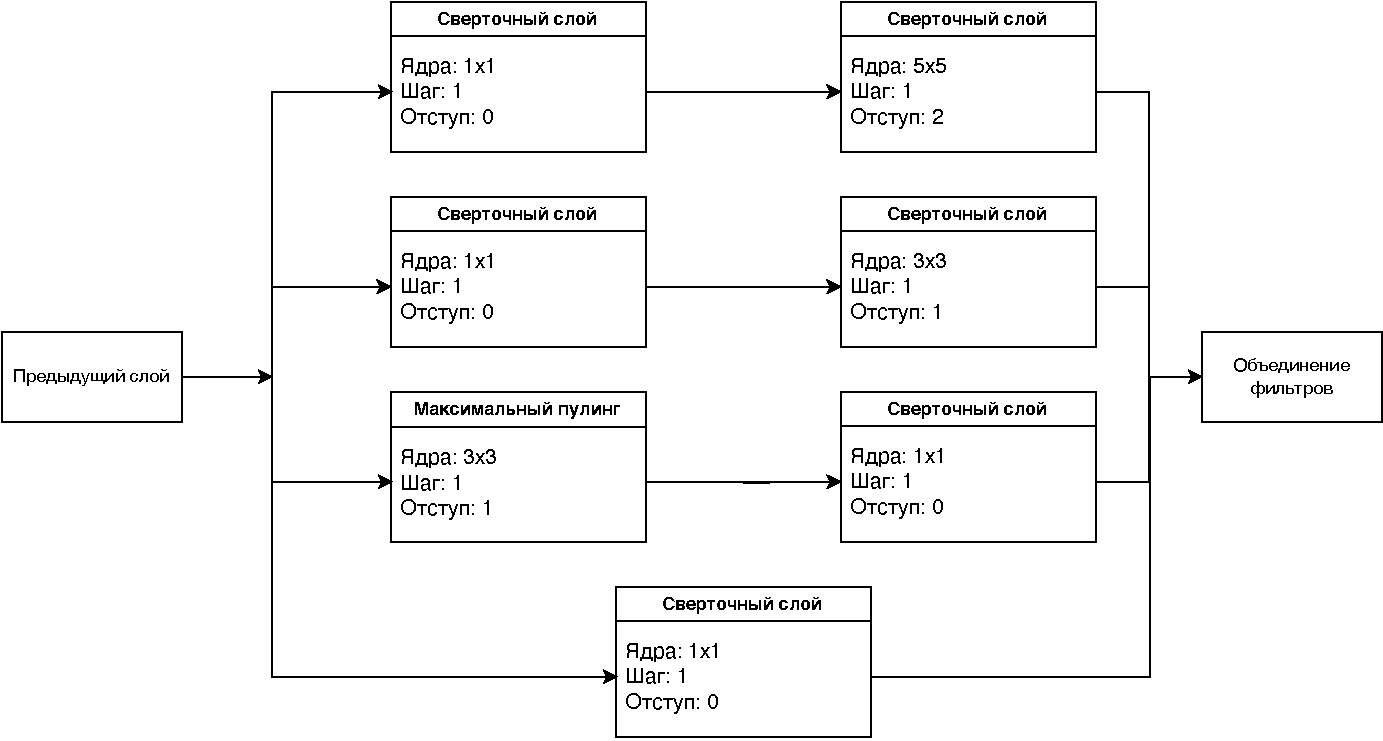
\includegraphics[width=\textwidth]{img/inception.pdf}
	\caption{Структура $inceptionV1$}
	\label{fig:inception}
\end{figure}

\begin{figure}[hbtp]
	\centering
	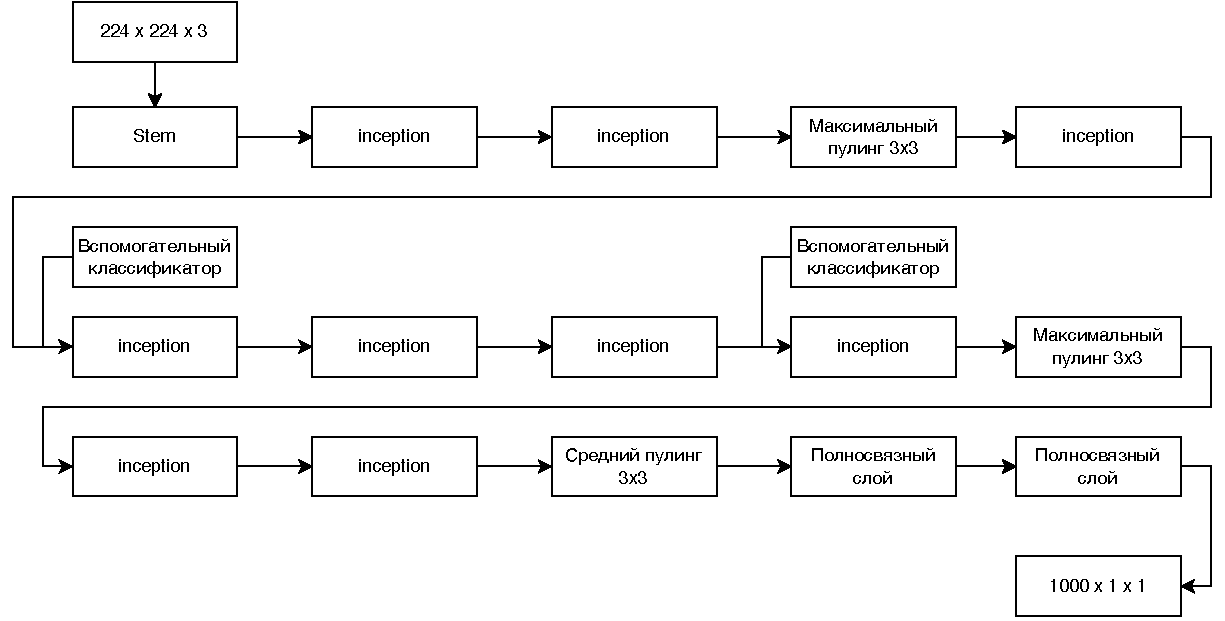
\includegraphics[width=\textwidth]{img/googlenet.pdf}
	\caption{Принцип работы GoogleNet}
	\label{fig:googlenet}
\end{figure}

\begin{figure}[hbtp]
	\centering
	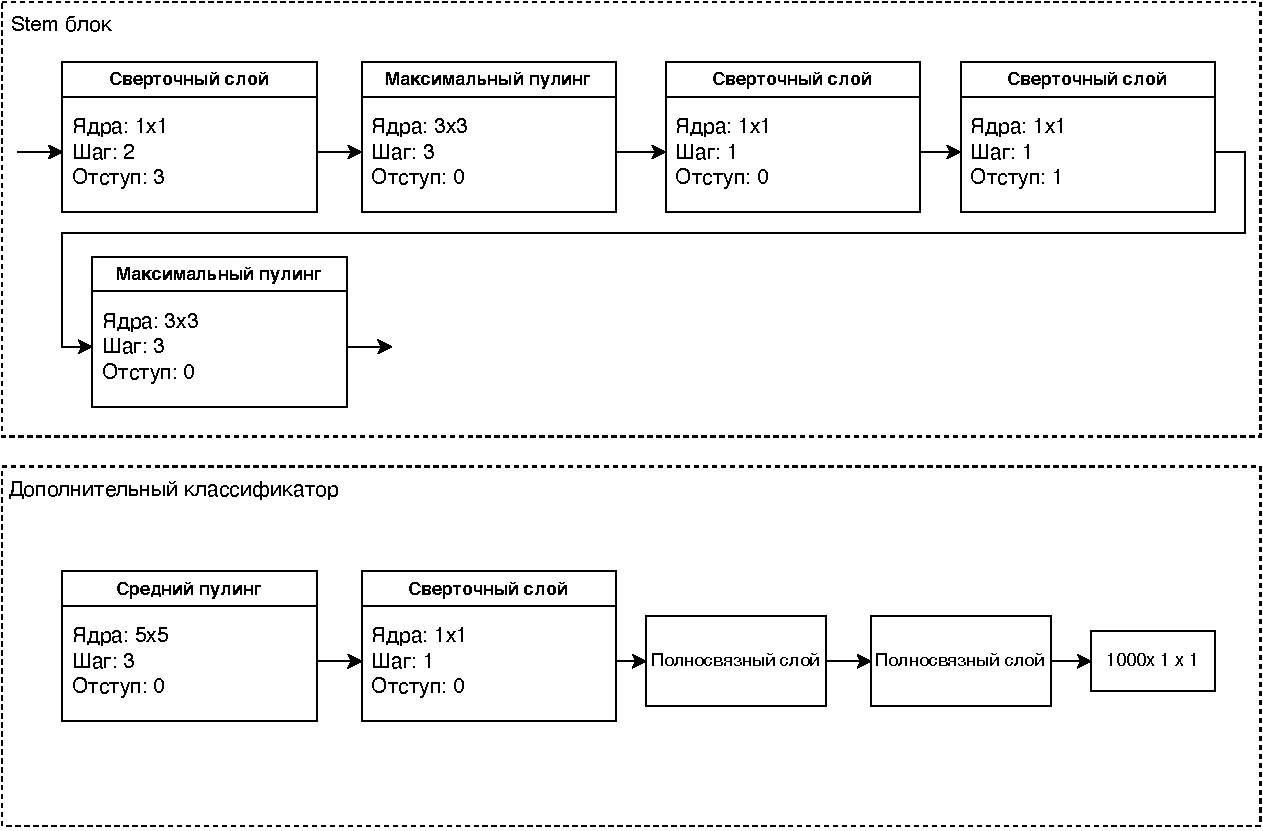
\includegraphics[width=\textwidth]{img/stem_aux.pdf}
	\caption{Структура $Stem$ блока и вспомогательного классификатора}
	\label{fig:stem_aux}
\end{figure}
\clearpage

\subsubsection{ResNet}
ResNet (от англ. Residual Network) - это остаточная сеть.  Считалось, что чем глубже сеть, тем больше информации можно получить, и тем устойчивее будут характеристики. Однако эксперименты показывают, что по мере углубления сети эффективность оптимизации ухудшается, а точность на тестовых и обучающих данных снижается. Это явление является результатом проблем расширения градиента и исчезновения градиента, вызванных углублением сети \cite{gradient_problem}.

 Для решения проблемы дегенерации в глубоких сетях можно искусственно заставить определенные слои нейронной сети пропустить соединение нейронов в следующем слое и соединить их в чередующихся слоях, ослабляя сильную связь между каждым слоем. Такие нейронные сети называются остаточными сетями (ResNet).
 
 Как показано на рисунке \ref{fig:resnet}, входные данные $x$ складываются с оригинальными данными $x$, и после обработки сверточным слоем получается $F(X)$, в сравнении с традиционной структурой CNN. Впоследствии можно одновременно сохранить действительную информацию двух слоев, и одновременно снизить потерю информации, вызванную слишком большим количеством слоев. Модель CNN, построенная с использованием этой остаточной сети, может содержать 100 и более слоев. Модель, рассматриваемая в данной работе -- ResNet101, которая имеет 101 слой и 44 миллиона параметров.
 
 \begin{figure}[hbtp]
 	\centering
 	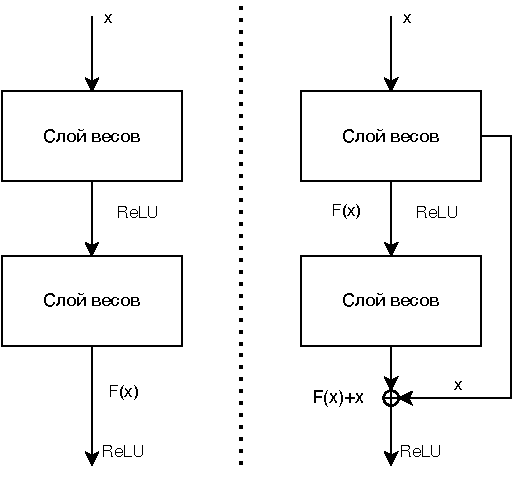
\includegraphics[width=\textwidth]{img/resnet.pdf}
 	\caption{Сравнение обычного обучения CNN (слева) и остаточного обучения (справа)}
 	\label{fig:resnet}
 \end{figure}
 \clearpage
 
 \subsubsection{Cравнение рассмотренных методов}
 Сравнительная характеристика рассмотренных методов представлена в
 таблице \ref{tab:compr}. 
 
\begin{table}[h]
 	\centering
 	\caption{Сравнение методов распознавания образов}
 	\label{tab:compr}
 	\resizebox{\textwidth}{!}{%
 		\begin{tabular}{|l|l|l|l|l|}
 			\hline
 			\textbf{Критерий}                     			& \textbf{AlexNet} & \textbf{VGG-16} & \textbf{GoogleNet} &  \textbf{ResNet101}\\ \hline
 			Время вычисления (сек)            			& 56       & 212                            & 77       					 & 197            \\ \hline
 			Точность на тестовых данных (\%)   & 86.67           & 85.19                & 94.81                  &     90.37       \\ \hline
 			FLOPs  														& 727           & 16000                 & 2000                   &    7600      \\ \hline
 		\end{tabular}%
 	}
\end{table}

FLOPs ---  количество операций с плавающей точкой (от англ. floating point operations), отражающее сложность вычислений.

Значения критериев для каждого из методов взяты из исследования <<A Comparative Study of Different CNN Models and Transfer Learning Effect for Under-water Object Classification in Side-Scan Sonar Images>> \cite{models-comprasion}.

Из представленной таблицы можно сделать вывод: GoogleNet является наиболее подходящей моделью, так как является наиболее точной, к тому же по времени вычисления и FLOPs она незначительно уступает AlexNet, в сравнении с VGG и ResNet имеет лучшие показатели по всем критериям.

\subsection{Формализация постановки задачи}
На основе рассуждений, представленных в данном разделе, можно сделать вывод, что для оценки безопасности водителя требуется:
\begin{itemize}[leftmargin=1.6\parindent]
	\item[--] видео или множество фотографий из салона автомобиля;
	\item[--] обученная модель нейронной сети;
	\item[--] значения весов для каждого действия водителя;
	\item[--] алгоритм вычисления коэффициента безопасности водителя на основе количества полученных действий и весов.
\end{itemize}

Формально данная задача может быть описана с помощью IDEF0-диаграммы нулевого уровня, представленной на рисунке \ref{fig:idef0}.
 \begin{figure}[hbtp]
	\centering
	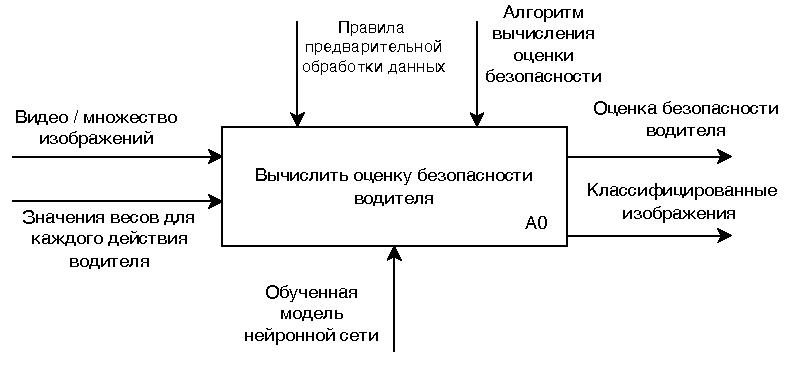
\includegraphics[width=\textwidth]{img/idef0.pdf}
	\caption{Постановка задачи в виде IDEF0-диаграммы нулевого уровня}
	\label{fig:idef0}
\end{figure}
\clearpage

\subsection*{Вывод}
В данном разделе была рассмотрена задача оценки безопасности водителя, которая может быть сведена к задаче классификации изображений. Также были описаны сверточные нейронные сети и их архитектура, рассмотрены технологии классификации изображений на основе сверточных нейронных сетей.

В качестве базовой технологии для разрабатываемого метода была выбрана модель сверточной нейронной сети GoogleNet, так как имеет наилучшую точность, в сравнении с другими рассмотренными методами, а также сравнительно небольшую сложность и время вычисления.

Также была формализована задача с помощью  IDEF0-диаграммы нулевого уровня.

\pagebreak